\documentclass{article}
\usepackage{iclr2026_conference,times}
\usepackage{graphicx}
\usepackage{amsmath}
\usepackage{amssymb}
\usepackage{amsthm}

\graphicspath{{../figures/}}

\title{Trajectory-Token Support Sieves for Reward-Token Tail Audits}

\author{Anonymous Authors}

\newtheorem{proposition}{Proposition}

\begin{document}
\maketitle

\begin{abstract}
Trajectory Transformers plan by decoding interleaved state, action, and reward tokens. This paper audits a token-level failure mode that is easy to miss when a planner only tracks predicted return: score-only candidate selection can raise decoded reward-token sums while moving the selected sequence into low-support prefixes and dynamically inconsistent state transitions. We study this mechanism in a reproducible discretized autoregressive surrogate that preserves the Trajectory Transformer planning interface while making every token probability inspectable. The main diagnostic treats the full trajectory token string as the selected object and measures average log-likelihood, maximum prefix surprise, token-level dynamics inconsistency, selected-mode collapse, and realized simulator return. In the horizon-stress control, score-only selection from 64 candidates raises predicted return by 5.572 relative to a single candidate while realized return drops by 7.553. A Support-Calibrated Plan Sieve improves realized return by 5.455 at the same candidate count or blocks unsafe candidate sets. The evidence is synthetic and mechanism-focused; benchmark neural Trajectory Transformer validation is left as the next step.
\end{abstract}

\section{Introduction}

Sequence modeling has become a compelling lens for offline reinforcement learning. Decision Transformers condition action generation on desired return \citep{chen2021decision}, while Trajectory Transformers (TTs) model full trajectories and decode high-reward continuations with beam-style planning \citep{janner2021trajectory}. This paper studies a narrow but important failure mode: what happens when the inference procedure increases the number of candidate trajectory strings scored by the model?

Score-only selection is attractive because it is simple: decode many candidates, score them, and execute the highest-scoring one. In preference learning, related procedures can overoptimize imperfect reward models \citep{gao2023scaling}. For TTs, the problem is more structured. The reward being optimized is not only an external scalar; reward tokens are part of the autoregressive sequence alongside state and action tokens. This suggests a TT-specific failure: increasing the candidate count can select a string whose reward tokens are extreme even though its prefixes are surprising and its decoded state transitions do not match the dynamics implied by its decoded actions.

We call this \emph{reward-token extremization}. The contribution is a diagnostic and repair for this architecture-specific mechanism, not a claim about broad benchmark performance.

\section{Setup}

A trajectory token string has the repeated layout
\[
(s_0,a_0,r_0,s_1,a_1,r_1,\ldots,s_{H-1},a_{H-1},r_{H-1}).
\]
The surrogate model factorizes it autoregressively,
\[
p_\theta(x_{1:3H})=\prod_{t=1}^{3H} p_\theta(x_t \mid x_{<t}),
\]
using smoothed context counts over discretized state, action, and reward vocabularies. This n-gram surrogate is intentionally inspectable. It preserves the TT planning interface while keeping every diagnostic reproducible.

Candidate score is the decoded reward-token sum
\[
S(x)=\sum_{t=0}^{H-1}\hat r_t.
\]
Realized utility \(U(x)\) is measured by executing the decoded action sequence in the ground-truth simulator from the same initial state. The diagnostic also records average token log-likelihood, maximum prefix negative log-probability, and a dynamics inconsistency score:
\[
D(x)=\frac{1}{H-1}\sum_{t=0}^{H-2}
\left| \hat s_{t+1}-f(\hat s_t,\hat a_t)\right|.
\]

\section{Finite-Candidate Selection Identity}

\begin{proposition}[Exact score-selected utility identity]
Let candidates \(X_1,\dots,X_K\) be i.i.d. from a finite distribution over outcomes \(i\) with probability \(p_i\), proxy score \(s_i\), and realized utility \(u_i\). Select a maximum-score candidate and break ties uniformly among tied samples. Define \(p_{=i}=\Pr(s(X)=s_i)\) and \(p_{<i}=\Pr(s(X)<s_i)\). Then
\[
\Pr(\hat X_K=i)
=
K p_i \sum_{m=0}^{K-1}
\binom{K-1}{m}
\frac{p_{=i}^{m} p_{<i}^{K-1-m}}{m+1}.
\]
Consequently,
\[
\mathbb E[U(\hat X_K)]=\sum_i u_i \Pr(\hat X_K=i).
\]
\end{proposition}

The proof distinguishes one sampled copy of outcome \(i\). It is selected when no other sample has a higher score; if \(m\) other samples tie its score, the distinguished copy wins tie-breaking with probability \(1/(m+1)\). The remaining samples must have equal or lower score.

The consequence used in this paper is conditional. If a higher proxy-score tail has lower realized utility than the lower-score mass and its selection probability rises with candidate count, then expected selected utility can decrease as more candidates are scored. This does not say more decoding is always harmful; it says that proxy-score tails need utility alignment, not only high proxy score.

\section{Support-Calibrated Plan Sieve}

The repair calibrates thresholds on offline training trajectories. A candidate is accepted only if its average log-likelihood is above a low quantile, its maximum prefix surprise is below a high quantile, and its dynamics inconsistency is below a high quantile. Accepted candidates are ranked by a calibrated score:
\[
S_{\mathrm{sieve}}(x)=S(x)-\lambda_\ell[\tau_\ell-\ell(x)]_+
-\lambda_p[P(x)-\tau_p]_+
-\lambda_d[D(x)-\tau_d]_+.
\]
If no candidate is accepted, the planner returns the lowest-risk candidate and marks the candidate set as blocked. An adaptive candidate-count gate stops increasing the candidate set once the risk rate exceeds the calibrated ceiling.

The oracle real-utility selector appears only as an upper-bound diagnostic and is not a deployable method.

\section{Experiments}

The environment is a one-dimensional control problem with a support-limited high-return corridor. Offline behavior mostly visits safe moderate-return actions and rarely visits high-return trajectories. The model is trained only from this offline data. We run candidate counts \(K\in\{1,2,4,8,16,32,64\}\) and evaluate four controls: in-support, out-of-support, anti-aligned scorer, and horizon stress.

\begin{table}[t]
\caption{Summary from \texttt{results/summary.json}. Predicted and realized changes compare score-only selection at candidate count 64 to candidate count 1. The repair column reports sieve minus score-only realized return at candidate count 64.}
\label{tab:summary}
\begin{center}
\begin{tabular}{lccc}
\hline
Control & Predicted change & Realized change & Sieve repair \\
\hline
In support & 3.188 & -0.969 & 2.002 \\
Out of support & 4.233 & 2.941 & 1.673 \\
Anti-aligned scorer & 2.870 & -1.392 & 2.664 \\
Horizon stress & 5.572 & -7.553 & 5.455 \\
\hline
\end{tabular}
\end{center}
\end{table}

\begin{figure}[t]
\centering
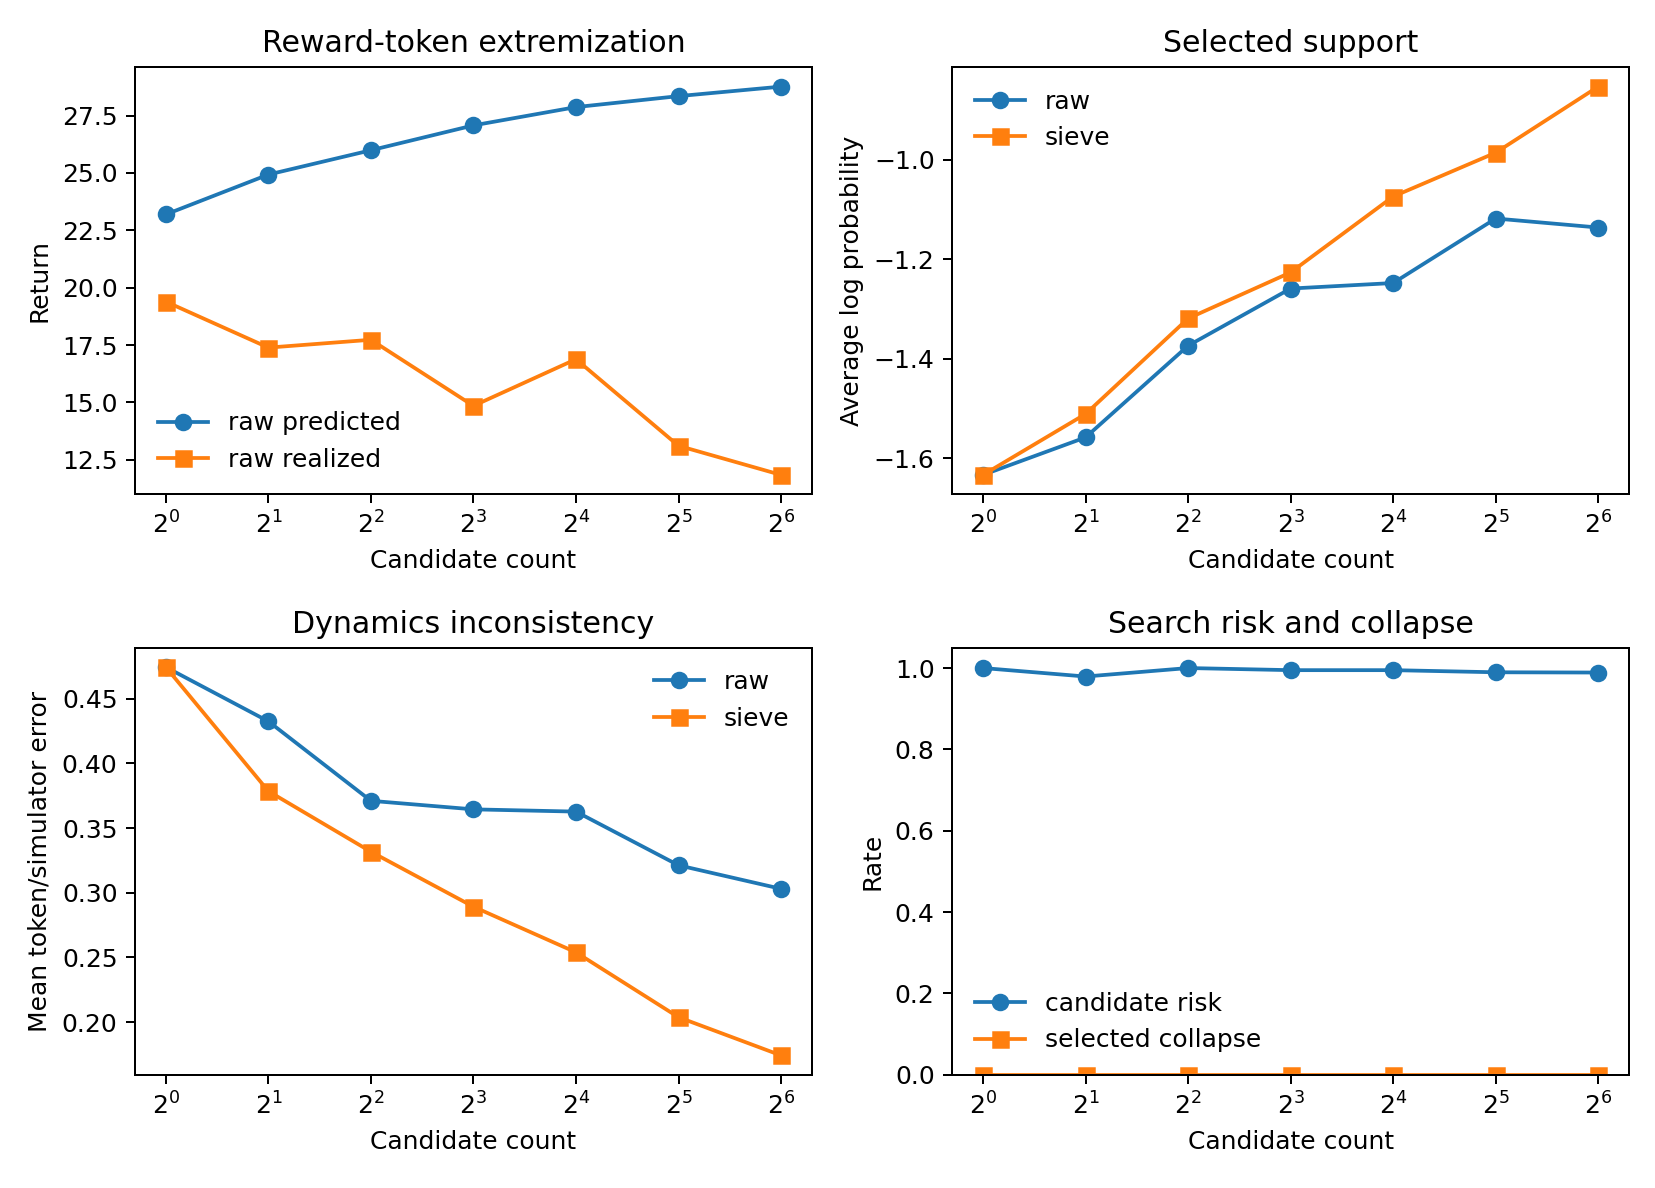
\includegraphics[width=\linewidth]{reward_extremization.png}
\caption{Horizon-stress control. Score-only selection raises predicted reward-token return while selected support and dynamics consistency deteriorate. The sieve keeps selected plans closer to calibrated support.}
\label{fig:extremization}
\end{figure}

\begin{figure}[t]
\centering
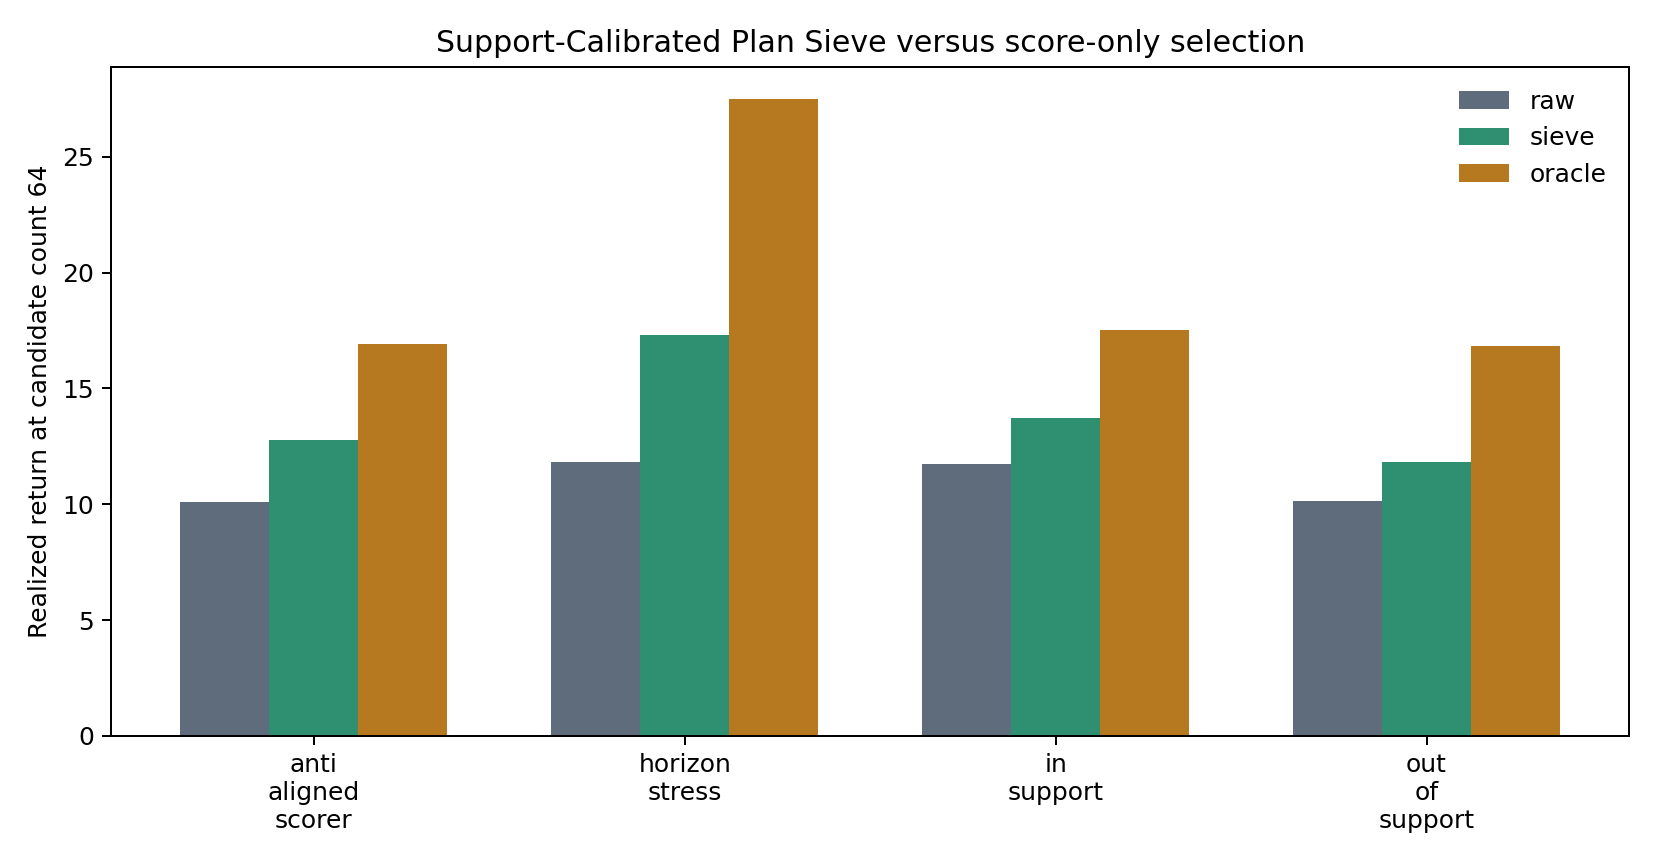
\includegraphics[width=0.86\linewidth]{repair_comparison.png}
\caption{Realized return at candidate count 64. The oracle is an upper-bound diagnostic; the deployable comparison is score-only selection versus the Support-Calibrated Plan Sieve.}
\label{fig:repair}
\end{figure}

\begin{figure}[t]
\centering
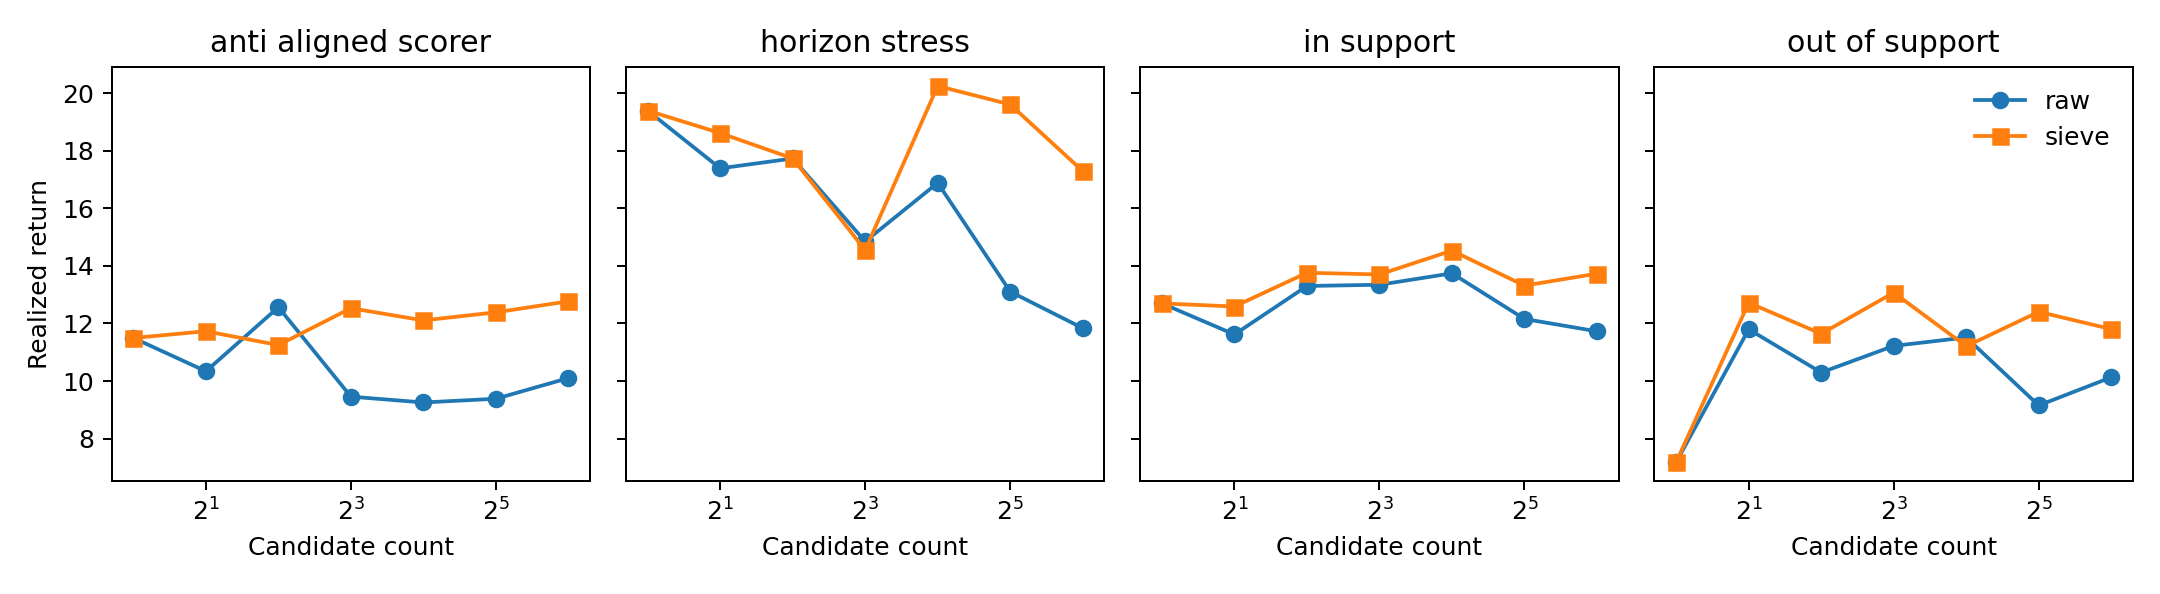
\includegraphics[width=0.92\linewidth]{control_panels.png}
\caption{Controls across candidate counts. The in-support setting is less fragile, while out-of-support and horizon-stress settings expose the selection-risk mechanism.}
\label{fig:controls}
\end{figure}

\begin{figure}[t]
\centering
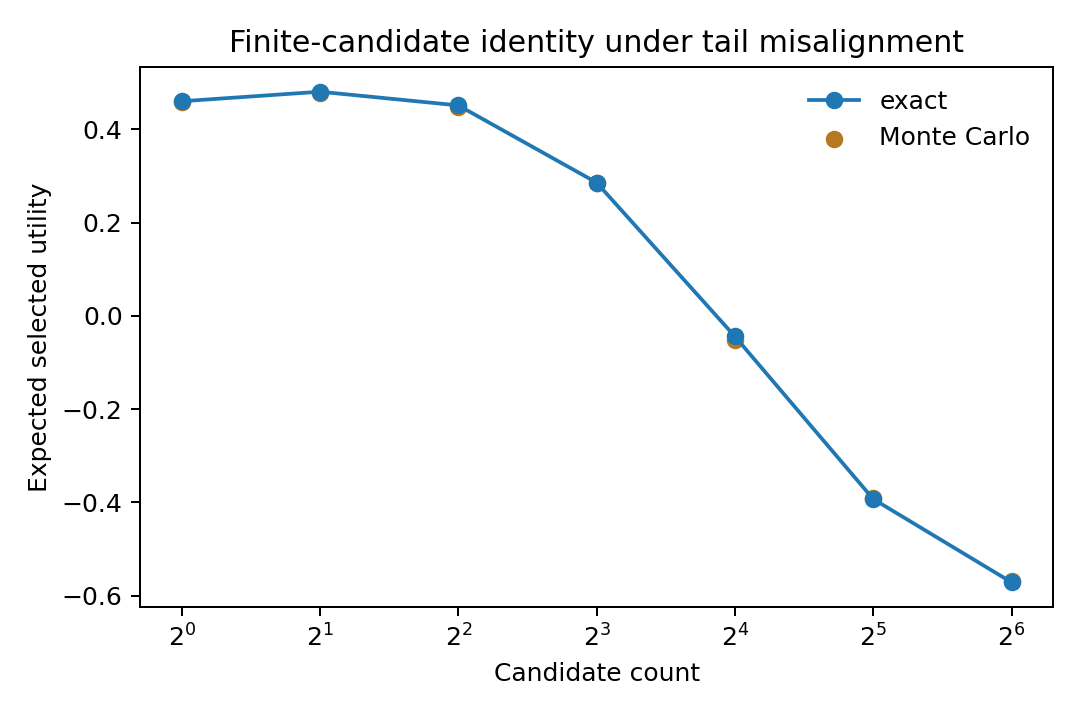
\includegraphics[width=0.70\linewidth]{exact_law_validation.png}
\caption{The finite-candidate identity matches Monte Carlo in a tail-misalignment example where larger candidate counts lower expected selected utility.}
\label{fig:law}
\end{figure}

\section{Discussion}

The results support a mechanism claim: score-only TT planning can optimize reward tokens into low-support token strings. The key observation is that the selected object is not merely an action plan but an autoregressive sequence whose prefixes and state-token transitions can be audited. A generic reward reranker would miss that structure.

The main limitation is scale. The current implementation is synthetic and uses an interpretable surrogate rather than a neural Transformer. This is appropriate for an adversarial first pass because exact probabilities and support diagnostics can be inspected, but it is not a substitute for neural TT experiments on standard offline RL benchmarks. Future work should train a TT on D4RL-style data, compare sampling and deterministic beam variants, and test whether the same prefix-surprise and dynamics-consistency signals predict failure in larger models.

\section{Reproducibility}

The repository includes the simulator, token model, experiments, figures, tests, claim audit, proof audit, and this paper source. The primary commands are:

\begin{verbatim}
python -m trajectory_token_sieve.experiments.run_smoke
python -m trajectory_token_sieve.experiments.run_all
pytest
\end{verbatim}
The claim-audit entry point is \texttt{run\_claim\_audit} in the same experiments package.

\bibliography{references}
\bibliographystyle{iclr2026_conference}

\appendix
\section{Claim Boundary}

The paper makes a synthetic mechanism claim. It does not claim top benchmark performance, deployment readiness, or universal failure for every Trajectory Transformer. The final audit in the repository lists the strongest result, the strongest repair result, and the remaining weaknesses.

\end{document}
